% presentation
%\documentclass{beamer}

% handout
\documentclass[handout]{beamer}

%\includeonly{preface}

\mode<beamer>{
  \usetheme{Frankfurt}
  \mode<presentation>
}

\mode<handout>{
  \usepackage{pgfpages}
  \pgfpagesuselayout{2 on 1}[a4paper]
}

\usepackage{tikz}
\usetikzlibrary{mindmap,trees}

% other themes
%\usepackage{beamerthemeWarsaw}
%\usepackage{beamerthemeBoadilla}
%\usepackage[compress]{beamerthemeSingapore}


% layout settings
\setbeamertemplate{blocks}[rounded][shadow=false]
\setbeamertemplate{navigation symbols}{}
\setbeamersize{text margin left = 4mm}
\setbeamersize{text margin right = 4mm}
\setbeamercovered{transparent}

% other packages
%\usetheme[Boadilla]{}
\usepackage{calc}
\usepackage[ruled]{algorithm2e}
\usepackage{stmaryrd}
%

%\usepackage{tabularx,booktabs}
\usepackage{booktabs}
%\useinnertheme{rounded}
\usecolortheme{dolphin}
\usecolortheme{rose}
%\setbeamercolor{title}{fg=black,bg=white!80!black}
\setbeamercolor{title}{fg=black,bg=white!80!blue}
\usefonttheme[onlysmall]{structurebold}


\usepackage{colortbl}

\usepackage{listings}


\definecolor{lightgray}{gray}{0.9} \lstset{backgroundcolor=\color{lightgray}}
\lstdefinelanguage{rock}{morekeywords=
  {mean,std,hist,save,load,rotate,min,max,get,
	scale,union,delete,degree,kernel,gethw,getparameter,bandwidth,
    symmetry,Miller,Miller2quat,uniformODF,unimodalODF,fibreODF,xvector,yvector,zvector,
    loadPoleFigure,PoleFigure,plot,plotpdf,plotipdf,calcODF,vector3d,cross,norm,
    dot,sum,savefigure,plotDiff,calcerror,
    quaternion,idquaternion,dist,Laue,length,angle,add,subGrid,refine,GridLength,getResolution,getRho,
    polar,S2Grid,santafee,mix2,modalorientation,fourier,textureindex,entropy,volume,
    fibrevolume,uiimport,scatter,cif2symmetry,remove_outlier,
    simulatePoleFigure,SimulateEBSD,grainfun,hold,getFundamentalRegion,symvec,
    FourierODF,find_outlier,bar,copyproperty,plotspatial,hasholes,principalcomponents,
    hullprincipalcomponents,loadEBSD,segment2d,plotboundaries,plotodf,plotspatial,area,
    aspectratio,grain,grainfun,grainsize,get,plotgrains,plotellipse,plotsubfractions,plotboundary,
    hasholes,hassubfraction,hullarea,hullcentroid,hullperimeter,centroid,borderlength,
    deltaarea,equivalentperimeter,perimeter,joincount,link,misorientation,neighbours,
    paris,shapefactor,toebsd,rotation,axis,Euler,symmetrise,orientation,eq,inverse,BinghamODF,set,
    project2FundamentalRegion,annotate},
  sensitive=false, morestring=[b][\emph]', moredelim=[is][\alert]{/+}{+/},
  morecomment=[s][\emph]{<options}{>}, morecomment=[l]{\%},
  commentstyle=\color{darkgray} }

\lstset{language=rock}
\lstset{emph={symmetries,concentration},emphstyle={\bf \color{white!25!black}}}


\newtheorem{Remark}{Remark}
\newtheorem{Proposition}{Proposition}
\renewcommand{\O}{\mathcal O}
\newcommand{\PGroup}{S_\text{Point}}
\newcommand{\Y}{\mathcal Y}
\renewcommand{\angle}{\measuredangle}
\newcommand{\mtex}{{\large \bf{\color{red}M}TEX\,}}%
\newcommand{\MTEX}{{\bf {\color{red}M}TEX\,}}%
\newcommand{\degree}{\ensuremath{^\circ}}   % Gradzeichen
%\newcommand{\degree}{^\circ}
\newcounter{exercisescounter}
\newenvironment{Exercise}{\refstepcounter{exercisescounter}%
  \begin{block}{Exercise \arabic{exercisescounter}}}
  {\end{block}}


\author{R. Hielscher\inst{1} \and H. Schaeben\inst{2} \and F. Bachmann\inst{2}}

\title{{\Huge \bf{\color{red}M}TEX}}
\subtitle{A Texture Calculation Toolbox}
%\titlegraphic{\includegraphics[width=1.5cm]{pic/tu_logo}}

\institute{\inst{1}Faculty of Mathematics,\\
	Chemnitz University of Technology, Germany
	\and
  \inst{2}Geoscience Mathematics and Informatics,\\
  Freiberg University of Mining and Technology, Germany}

\date{18 March 2010}


\begin{document}


\frame[plain]{\titlepage}

\mode<handout>{
 \frame[plain]{}
}

\section{MTEX}


\begin{frame}{What is \MTEX: some numbers and facts}


\begin{block}{}

%\mindmap?
\begin{itemize}
\item developed since 2007
\item 25000 lines of matlab code in over 900 m-files
\item 15000 lines comments
\item 750 help pages
\item 5 reference papers
\item support for 20 pole figure and 5 EBSD data formats
\end{itemize}
\end{block}

\begin{block}{}
  \vspace*{0.25em}
  \hspace{1.25em}
  \begin{tabular}{lll}
    version & release date & downloads \\
    \toprule
    mtex 1.0 & June 2008 & $900$ \\
    mtex 2.0 & October 2009 & $800$ \\
    mtex 3.0 & August 2010 & $650$\\
    mtex 3.2 & May 2011 &
  \end{tabular}
\end{block}


\end{frame}



\begin{frame}
  \frametitle{Feature Overview}

 \renewcommand{\arraystretch}{1.25}
 \begin{center}

  \begin{tabular}{p{3cm} p{8cm}}
    Classes & Methods \\
    \toprule
    \rowcolor{blue!10}
    Crystal Geometry & crystal symmetries, CIF files, Miller indices, Euler angles, orientations,
    missorientations\\
    ODF & model ODFs, pole figures, inverse pole figures, volume portions,
    modal orientations, texture index\\
    \rowcolor{blue!10}
    Pole Figures & outliers, ODF estimation, error analysis\\
    EBSD  & orientation statistics, ODF estimation, grain detection,
    missorientation analysis\\
    \rowcolor{blue!10}
    Grains & volume, surface, neighbors, mean orientation, missorientation\\
    Tensors& elasticity tensors, Young's
    modulus, shear modulus, Poisson's ratio, linear compressibility,
    wave velocities
  \end{tabular}
  \end{center}
 \end{frame}


%%% Local Variables:
%%% mode: latex
%%% TeX-master: "main"
%%% End:


\section{MATLAB}

\subsection*{Vectors and Matrixes}


\begin{frame}[fragile]
  \frametitle{Vectors and Matrixes}

Define vectors:

\begin{lstlisting}
v = [1;2;3;4];     % a vertical vector
h = [1 2 3 4];     % a horizontal vector
M = [[1;2] [3;4]]; % a 2x2 Matrix
s = 1:4;           % the same as h
\end{lstlisting}

Calculate with vectors:
\begin{lstlisting}
u = 5 * v    % multiply vectors by a scalar
w = u - v    % subtract two vectors
x = u .* v   % componentwise multiplication
y = [u v]    % concatenation of vectors
\end{lstlisting}

Example: polar to Euclidean coordinates
\begin{lstlisting}
x = sin(theta) .* cos(rho)
y = sin(theta) .* sin(rho)
\end{lstlisting}

\end{frame}

\subsection*{Indexing of Vectors}

\begin{frame}[fragile]
  \frametitle{Vectors}


Indexing by numbers:

\begin{lstlisting}
v(1)     % the first element
v(2:end) % the last three elements
M(2,1)   % the bottom left element
M(:,2)   % the second column
\end{lstlisting}

Indexing by conditions:

\begin{lstlisting}
v( v > 1 )   % all elements that are larger then 1
v( u == v)   % all elements where u and v coincides
\end{lstlisting}

Changing elements

\begin{lstlisting}
v(1:3) = 1       % set the first three elements to 1
v( v == 0 ) = [] % remove all zeros
\end{lstlisting}

\end{frame}

\subsection*{Working with Data}


\begin{frame}[fragile]
  \frametitle{A First Script}

Load raw pole figure data stored in a column formated ascii file and plot the
data as colorcoded circles.

\begin{lstlisting}
uiimport([mtexDataPath '/juelich/104.hem']);

theta = data(:,1);     % first row is polar angle
rho = data(:,2);       % second row is azimuth angle
intensity = data(:,3); % third row is intensity

scatter(rho,theta,50,intensity,'filled') % plot data

\end{lstlisting}

\center{\includegraphics[width=10cm]{pic/scatter}}

\end{frame}


\subsection*{Exercises}

\begin{frame}

  \begin{Exercise}
    \begin{enumerate}[a)]
      \item  Construct a vector \textbf{e} of all even numbers between 10 to 30.
      \item  Construct a vector \textbf{s} of the first 11 sqare numbers.
      \item  Set in \textbf{s} all values to 0 where \textbf{e} $>$ \textbf{s}!
    \end{enumerate}
  \end{Exercise}

  \begin{Exercise}
    \begin{enumerate}[a)]
    \item Load the file \texttt{data/juelich/104.hem} and plot the data as a
      scatter plot!
    \item Determin the minimum, maximum and mean
      intensity of the data!
    \item Plot a histogram of the intensities.
    \item Transform the data into cartesian coordinates and plot them!
    \item Remove all negative values from the data and plot them!
    \end{enumerate}
  \end{Exercise}
\end{frame}



%%% Local Variables:
%%% mode: latex
%%% TeX-master: "main"
%%% End:


\section{Geometry}



\subsection*{Vector3d}

\begin{frame}[fragile]
  \frametitle{Specimen Directions - The \MTEX Class \texttt{\bf vector3d}}

  Definition:

\begin{lstlisting}
v = vector3d(1,1,1);    % by Cartesian coordinate
v = sph2vec(theta,rho); % by polar coordinates
v = xvector;            % predefined vectors
\end{lstlisting}

  \medskip

  \begin{columns}
    \begin{column}{8.5cm}

      Calculations:

\begin{lstlisting}
v = [xvector,yvector]; w = v(1);
v = 2*xvector-yvector;
\end{lstlisting}

    \medskip

    Basic Functions:

\begin{lstlisting}
cross(v1,v2), dot(v1,v2)
norm(v), sum(v)
vec2sph(v)
\end{lstlisting}
  \end{column}
  \begin{column}{3cm}
   \includegraphics[width=3cm]{pic/vector3d}
  \end{column}
\end{columns}



\end{frame}

\subsection*{quaternion}


\begin{frame}[fragile]
  \frametitle{Rotations - The \MTEX Class \texttt{\bf quaternion}}

Definition:

\begin{lstlisting}
q = quaternion(a,b,c,d);
q = axis2quat(axis,omega);
q = euler2quat(alpha,beta,gamma);
q = euler2quat(phi1,Phi,phi2,'Bunge');
q = Miller2quat([h k l],[u v w],CS);
\end{lstlisting}
%q = idquaternion;

\medskip

\begin{columns}
  \begin{column}{8.5cm}

    Calculations:

\begin{lstlisting}
q = [q1,q2]; q1 = q(1)
q = q1 * q2; w = q * v
\end{lstlisting}

    \medskip

    Basic Functions:

\begin{lstlisting}
omega = rotangle(q)
v = rotaxis(q)
[alpha,beta,gamma]  = quat2euler(q)
\end{lstlisting}

  \end{column}

  \begin{column}{3cm}
    \includegraphics[width=3cm]{pic/quaternion}
  \end{column}

\end{columns}
\end{frame}

\subsection*{Symmetry}
\begin{frame}[fragile]
  \frametitle{Crystal Symmetries - The \MTEX Class \texttt{\bf symmetry}}

  Definition:

\begin{lstlisting}
S = symmetry('triclinic',[a,b,c],[alpha,beta,gamma])
S = symmetry('-3m',[a,b,c],/+'a||x'+/);
S = symmetry('O');
\end{lstlisting}

\medskip

\begin{columns}
  \begin{column}{8.5cm}

Load Symmetry from CIF file:

\begin{lstlisting}
cif2symmetry('quartz.cif')
\end{lstlisting}

\medskip

    Basic Functions:

\begin{lstlisting}
symmetriceVec(SS,v)
dist(CS,SS,q1,q2)
quaternion(CS)
getFundamentalRegion(CS)
\end{lstlisting}
  \end{column}

  \begin{column}{3cm}
    \includegraphics[width=3cm]{pic/sym}
  \end{column}

\end{columns}

\end{frame}

\subsection*{Miller}

\begin{frame}[fragile]
  \frametitle{Crystal Directions - The \MTEX Class \texttt{\bf Miller}}

  Definition:

\begin{lstlisting}
h = Miller(1,0,0,CS);
h = [Miller(1,1,-2,3,CS),Miller(0,1,-1,0,CS)]
h = vec2Miller(v,CS);
\end{lstlisting}

\medskip

\begin{columns}
  \begin{column}{8.5cm}

    Calculations:

\begin{lstlisting}
q * Miller(1,0,0,CS)
q * symeq(Miller(1,0,0,CS))
\end{lstlisting}

    \medskip

    Basic Functions:


    \begin{onlyenv}<1>
\begin{lstlisting}
symeq(h1,h2)
symvec(h)
angle(h1,h2)
plot([h1,h2],'all')
\end{lstlisting}
    \end{onlyenv}

    \begin{onlyenv}<2>
      \lstset{stringstyle=\color{red},emph={antipodal},emphstyle=\em\color{red}}
\begin{lstlisting}
symeq(h1,h2,`antipodal`)
symvec(h,`antipodal`)
angle(h1,h2,`antipodal`)
plot([h1,h2],'all',`antipodal`)
\end{lstlisting}
    \end{onlyenv}

  \end{column}

  \begin{column}{3cm}
    \includegraphics[width=3cm]{pic/miller}
  \end{column}

\end{columns}

\end{frame}

\subsection*{S2Grid}


\begin{frame}[fragile]
  \frametitle{Sets of Specimen Directions - The \MTEX Class \texttt{\bf S2Grid}}

Definition:

\begin{lstlisting}
S2G = S2Grid('regular','resolution',5*degree);
S2G = S2Grid('regular','maxrho',80*degree);
S2G = S2Grid('equispaced','points',10000);
\end{lstlisting}

\medskip

Basic Functions:

\begin{lstlisting}
add, delete, rotate, union, subGrid, refine,
GridLength, getResolution, getRho, getTheta,
polar, vector3d
\end{lstlisting}

\onslide<1->
\begin{center}
  \includegraphics[width=2.5cm]{pic/S2Grid1} \quad
  \includegraphics[width=2.5cm]{pic/S2Grid2} \quad
  \includegraphics[width=2.5cm]{pic/S2Grid3} \quad
  \includegraphics[width=2.5cm]{pic/S2Grid4}
\end{center}

\end{frame}

\subsection*{Exercises}

\begin{frame}

  \begin{Exercise}
    Consider trigonal crystal symmetry.

    \begin{enumerate}[a)]
    \item Find all crystallographic directions symmetrically equivalent to $h
      = (1, 0, \bar 1, 0)$ (Miller indices)!
    \item Find crystallographic directions such that the number of their
      crystallographic equivalent directions on the upper hemisphere (without
      equator) is 1, 3, or 6?
    \item Construct an orientation that rotates the crystallographic
      directions $(0,0,0,1)$ and $(2,\bar 1,\bar 1,0)$ onto the specimen
      directions $(1,0,0)$ and $(0,1,0)$, respectively.
    \item Find all crystallographic equivalent orientations to
      $(45\degree,0\degree,0\degree)$ (Euler angle) and give its Euler angles!
    \item Find all crystallographic equivalent specimen directions to the crystal
      direction $(1,1,\bar 2,1)$ under the orientation
      $(45\degree,0\degree,0\degree)$ (Euler angle)!
    \end{enumerate}

  \end{Exercise}

\end{frame}

%%% Local Variables:
%%% mode: latex
%%% TeX-master: "main"
%%% End:


\section{Model ODFs}


\subsection*{ODFs in MTEX}


\begin{frame}[fragile]
  \frametitle{Orientation Density Functions in \MTEX}


  \centering{
    \includegraphics[width=10cm]{latex_pic/odf}
  }

\end{frame}

\subsection*{ODFs in MTEX}


\subsection*{The Class kernel}


\begin{frame}[fragile]
  \frametitle{The Shape of the ODF -- The \MTEX Class \texttt{\bf kernel}}

Definition:

\begin{lstlisting}
psi = kernel('de la Vallee Poussin',80);
psi = kernel('Abel Poisson','halfwidth',10*degree);
\end{lstlisting}

\medskip

Supported kernel functions:

\begin{quote}
  Abel -- Poisson, de la Vall\'ee Poussin, von Mises -- Fisher, fibre von Mises
  -- Fisher, Gauss -- Weierstrass, Dirichlet, Bump
\end{quote}

Plot of the \textcolor{blue}{Abel Poisson}, the \textcolor{red}{Dirichlet} and
the \textcolor{green}{Bump} kernel:

\onslide<1->
\begin{center}
  \includegraphics[width=3.5cm]{pic/K} \quad
  \includegraphics[width=3.5cm]{pic/RK} \quad
  \includegraphics[width=3.5cm]{pic/Fourier}
\end{center}

\end{frame}

\subsection*{Unimodal ODFs}

\begin{frame}[fragile]
  \frametitle{Defining Unimodal ODFs in \MTEX}

\begin{columns}

  \begin{column}{8.5cm}

      Characteristics of an unimodal ODF:
      \begin{enumerate}
      \item crystal symmetry
      \item specimen symmetry
      \item modal orientation
      \item kernel function
      \end{enumerate}



\begin{lstlisting}
SS = symmetry('orthorhombic')
CS = symmetry('cubic')
q = Miller2quat([1 2 2],[2 2 1],CS);
psi = kernel('von Mises Fisher',...
             'halfwidth',20*degree);
\end{lstlisting}

      \begin{actionenv}<1-| alert@1->
\begin{lstlisting}
odf = unimodalODF(q,CS,SS,psi)
\end{lstlisting}
    \end{actionenv}

\end{column}

    \begin{column}{3cm}
      \onslide<1->
      \includegraphics[width=3cm]{pic/unimodalODF}
    \end{column}
  \end{columns}

\end{frame}



\subsection*{Fibre ODFs}

\begin{frame}[fragile]
  \frametitle{Defining Fibre ODFs in \MTEX}

  \begin{columns}

    \begin{column}{8.5cm}

      Characteristics of an Fibre ODFs:
      \begin{enumerate}
      \item crystal symmetry
      \item specimen symmetry
      \item crystal direction
      \item specimen direction
      \item kernel function
      \end{enumerate}


\begin{lstlisting}
SS = symmetry('triclinic')
CS = symmetry('hexagonal')
h = Miller(1,0,0,CS);
r = xvector;
psi = kernel('Abel Poisson',...
             'halfwidth',18*degree);
\end{lstlisting}

      \begin{actionenv}<1-| alert@1->
\begin{lstlisting}
odf = fibreODF(h,r,CS,SS,psi)
\end{lstlisting}
      \end{actionenv}

\end{column}

    \begin{column}{3cm}
      \onslide<1->
      \includegraphics[width=3cm]{pic/fibreODF}
    \end{column}
  \end{columns}


\end{frame}

\subsection*{Fourier ODFs}

\begin{frame}[fragile]
  \frametitle{Defining Uniform and  Fourier ODFs}

  The uniform ODF:
\begin{lstlisting}
SS = symmetry('triclinic')
CS = symmetry('hexagonal')
\end{lstlisting}

  \begin{actionenv}<1-| alert@1->
\begin{lstlisting}
 odf = uniformODF(CS,SS)
\end{lstlisting}
  \end{actionenv}

  \begin{block}{Fourier expansion of an ODF}
    \begin{equation*}
      f(\vec g) = \sum_{l=0}^L \sum_{k,k'=-l}^l C_l^{k,k'} T_l^{k,k'}(\vec g)
    \end{equation*}
    \begin{equation*}
      C = [C_0,C_1^{-1,-1},C_1^{0,-1},C_1^{1,-1},\ldots,C_1^{1,1},C_2^{-2,-2},\ldots,C_L^{L,L}]
    \end{equation*}
  \end{block}
The Fourier ODF:
  \begin{actionenv}<1-| alert@1->
\begin{lstlisting}
odf = FourierODF(C,CS,SS)
\end{lstlisting}
  \end{actionenv}



\end{frame}

\subsection*{ODF Arithmetic}

\begin{frame}[fragile]
  \frametitle{ODF Arithmetic}


  \begin{columns}
    \begin{column}{6cm}

      Calculate with ODFs:
\begin{lstlisting}
odf1 = unimodalODF(...)
odf2 = fibreODF(...)
odf3 = uniformODF(CS,SS)

odf = 0.2*odf1 + 0.3*odf2
      + 0.5*odf3

\end{lstlisting}

  Rotate ODFs:
\begin{lstlisting}
q = axis2quat(xvector,...
              90*degree);
odf = rotate(odf,q)
\end{lstlisting}


  Standard ODFs:
\begin{lstlisting}
odf = santafee;
\end{lstlisting}


\end{column}
\begin{column}{5cm}
  \includegraphics[width=5cm]{pic/santafeeh}
\end{column}
\end{columns}

\end{frame}

%%% Local Variables:
%%% mode: latex
%%% TeX-master: "main"
%%% End:


\section*{ODF Analysis}

\subsection*{Working with ODFs}

\begin{frame}
  \frametitle{Analyzing and Visualizing ODFs in \MTEX}

  \begin{center}
    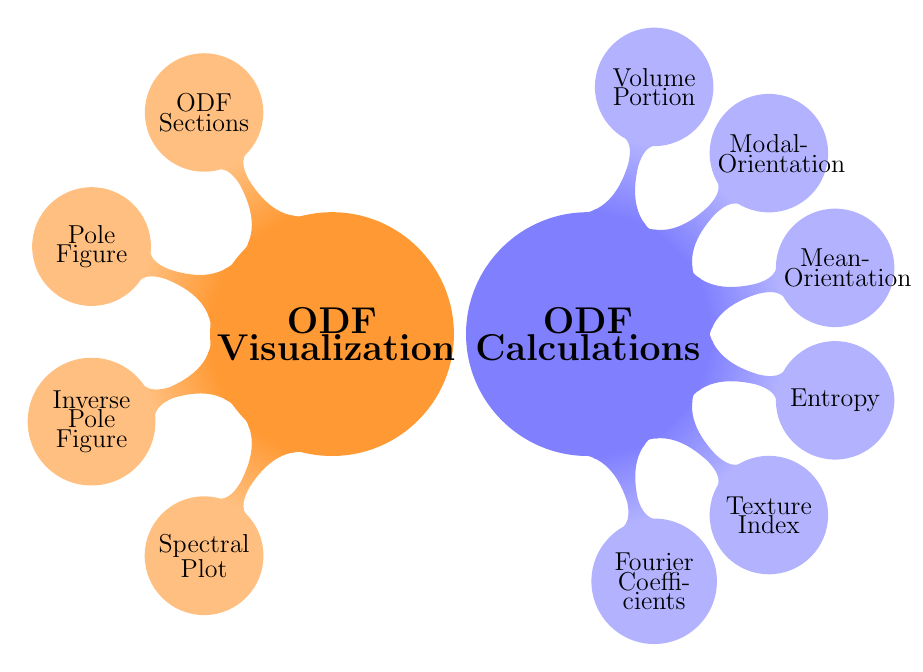
\begin{tikzpicture}[scale = 0.65,transform shape]
  \definecolor{myblue}{HTML}{92dcec}
  \tikzstyle{every annotation}=[fill=white, font=\sf]
  \tikzstyle{root concept}+=[text width=4.5cm]

  \path[mindmap, concept color=orange!80!]
  node[concept] {\huge \bf ODF\\ Visualization}
  child[grow = 120, concept color=orange!50]
  { node(ebsd) [concept](ebsd2) {\Large ODF Sections}}
  child[grow = 160, concept color=orange!50]
  { node[concept](pf) {\Large Pole Figure}}
  child[grow = -160, concept color=orange!50]
  { node[concept](pf) {\Large Inverse Pole Figure}}
  child[grow = -120, concept color=orange!50]
  { node[concept](pf) {\Large Spectral Plot}};

  \path[mindmap, concept color=blue!50!]
  node[concept] at (5,0){\huge \bf ODF \\Calculations}
  child[grow=75, concept color=blue!30]
  { node(ebsd) [concept](ebsd2) {\Large Volume Portion}}
  child[grow=45, concept color=blue!30]
  { node[concept](pf) {\Large Modal\-Orientation}}
  child[grow=15, concept color=blue!30]
  { node[concept](pf) {\Large Mean\-Orientation}}
  child[grow=-15, concept color=blue!30]
  { node[concept](pf) {\Large Entropy}}
  child[grow=-45, concept color=blue!30]
  { node[concept](pf) {\Large Texture Index}}
  child[grow=-75, concept color=blue!30]
  { node[concept](pf) {\Large Fourier Coefficients}};
\end{tikzpicture}
\end{center}

\end{frame}

\subsection*{Working with ODFs}

\begin{frame}[fragile]
  \frametitle{Texture Characteristics}

Comparing {\bf arbitrary} ODFs
\begin{lstlisting}
calcerror(odf1,odf2,'L1')  % 'RP', 'L2'
\end{lstlisting}


\pause

Preferred orientations:
\begin{lstlisting}
o = modalorientation(odf)  % the modal orientation
o = max(odf,n)             % find n relative peaks
o = mean(odf)              % the mean orientation
\end{lstlisting}


\pause

Volume portions:
\begin{lstlisting}
volume(odf,center,radius)   % the volume of a ball
fibrevolume(odf,h,r,radius) % the volume of a fibre
\end{lstlisting}

\pause

The shape of the ODF:
\begin{lstlisting}
textureindex(odf)          % the texture index
entropy(odf)               % the entropy
fourier(odf,order)         % the C-coefficients
\end{lstlisting}


\end{frame}


\subsection*{Plotting (Inverse) Pole Figures}

\begin{frame}[fragile]
  \frametitle{Plotting (Inverse) Pole Figures in \MTEX}

  General syntax:
\begin{lstlisting}
plotpdf(odf,Miller(0,1,0),<options>)
plotipdf(odf,[xvector,zvector],<options>)
\end{lstlisting}

Options:
\begin{lstlisting}
antipodal % add antipodal symmetry
complete  % plot complete sphere
\end{lstlisting}


\onslide<1->
\center{\includegraphics[height=3cm]{pic/ipdf}}

\end{frame}


\subsection*{Plotting an ODF}

\begin{frame}[fragile]
  \frametitle{Plotting  an ODF in \MTEX}

  \begin{columns}
    \begin{column}{6.5cm}
      General syntax:
\begin{lstlisting}
plot(odf,<options>)
\end{lstlisting}

      Sectioning:
      \lstset{emph={sigma},emphstyle={\color{blue}}}
\begin{lstlisting}
alpha, gamma, phi1, phi2
sigma, fibre
\end{lstlisting}

      Options:
\begin{lstlisting}
sections, center, resolution
\end{lstlisting}

      Example:
    \end{column}
    \begin{column}{5cm}
      \includegraphics[width=5cm]{pic/radialplot}
    \end{column}
  \end{columns}

\begin{lstlisting}
plot(odf,'fibre',{Miller(0,0,1),zvector},...
  'center',modalorientation(odf))
\end{lstlisting}

%\begin{lstlisting}
%plot(odf,'alpha',[45*degree])
%\end{lstlisting}

\end{frame}


\subsection*{Dubna}

\begin{frame}[fragile]
  \frametitle{A Sigma Plot of the Recalculated Dubna ODF in \MTEX}

\begin{lstlisting}
plot(rec,'sections',18,'FontSize',10)
\end{lstlisting}

\medskip

\includegraphics[width=\textwidth]{pic/ODFso9}

\end{frame}

\subsection*{SantaFe}

\begin{frame}[fragile]
  \frametitle{The Classical Plot of the SantaFe ODF in \MTEX}

\begin{lstlisting}
plot(SantaFe,'alpha','sections',18,...
     'projection','plain','gray','contourf')
\end{lstlisting}

\includegraphics[width=\textwidth]{pic/santafee}

\end{frame}

\subsection*{Exercises}

\begin{frame}

  \begin{Exercise}
    \begin{enumerate}[a)]
      \item Construct a cubic unimodal ODF with mode at $[0 0 1](3 1 0)$.
      \item What is its modal orientation in Euler angles?
      \item Plot some pole figures. Are there pole figures with and without
        antipodal symmetry? What about the inverse pole figures?
      \item Plot the ODF in $\sigma$ and $\phi_{2}$ - sections. How many modes
        do you observe?
      \item Compute the volume of the ODF that is within a distance of 10
        degrees of the mode. Compare the result with the uniform ODF.
    \end{enumerate}
  \end{Exercise}

  \begin{Exercise}
    \begin{enumerate}[a)]
    \item Construct a trigonal ODF that consists of two fibres at
      $h_1 = (0,0,0,1)$, $r_{1} = \mathbf{y}$, $h_2 = (1,0,\bar 1,0)$, $r_{2} = \mathbf{x}$.
    \item Do the two fibres intersect?
    \item What is the modal orientation of the ODF?
    \item Plot the ODF in $\sigma$ and $\phi_{2}$ - sections. How many
      fibres do you observe?
    \item Compute the texture index of the ODF.
    \end{enumerate}
  \end{Exercise}

\end{frame}


%%% Local Variables:
%%% mode: latex
%%% TeX-master: "main"
%%% End:


\section{Pole Figures Analysis}

\subsection*{Layout}

\begin{frame}[fragile]
  \frametitle{Experimental Pole Figures in \MTEX}

  \begin{columns}

    \begin{column}{8.2cm}

      Characteristics of a single experimental pole figure in \mtex:
      \begin{enumerate}
      \item crystal symmetry
      \item specimen symmetry
      \item list of specimen directions
      \item (list of superposed) crystal direction(s)
      \item (structure coefficients)
      \item list of diffraction intensities
      \item background radiation intensities (optional)
      \end{enumerate}

    \end{column}

    \begin{column}{3cm}
      \includegraphics[width=3cm]{pic/pf1}\\
      \includegraphics[width=3cm]{pic/pfso9_bg}
    \end{column}


  \end{columns}


\end{frame}


\subsection*{Import Wizard}



\begin{frame}[fragile]
  \frametitle{Importing Pole Figure Data - The Import Wizard}

  Formats supported by \MTEX:

  \begin{columns}

    \begin{column}{4cm}
      \begin{itemize}
      \item Popla: *.EPF
      \item BearTex: *.XPa
      \item Philips: *.txt
      \item generic ascii files
      \end{itemize}
    \end{column}

    \begin{column}{4cm}
       \begin{itemize}
      \item Aachen: *.exp
      \item J\"ulich: *.hem
      \item Geesthacht
      \item Dubna: *.cnv, *.cns
      \end{itemize}
    \end{column}

    \begin{column}{3cm}
       \begin{itemize}
      \item *.nja
      \item *.ptx
      \item *.plf
      \item *.xrdml
      \end{itemize}
    \end{column}

  \end{columns}


  \centerline{\includegraphics[width=6cm]{pic/iw}}
\end{frame}

\subsection*{Construction (high level)}

\begin{frame}[fragile]
  \frametitle{Importing Pole Figure Data Using a Script}

  \begin{columns}
    \begin{column}{8.5cm}

Script generated by the import wizard:

\begin{lstlisting}
CS = symmetry('-3m',[1.2 1.2 3.5]);
SS = symmetry('triclinic');
\end{lstlisting}

\pause

\begin{lstlisting}
pf_files = {'Q(10-10).cnv',...
            'Q(10-11)(01-11).cnv'}

h = {Miller(1,0,-1,0,CS),...
     [Miller(0,1,-1,1,CS),...
      Miller(1,0,-1,1,CS)]}

c = {1,[0.52,1.23]};
\end{lstlisting}

\pause

      \begin{actionenv}<1-| alert@1->
\begin{lstlisting}
pf = loadPoleFigure(pf_files,h,...
       CS,SS,'superposition',c);
\end{lstlisting}
      \end{actionenv}

    \end{column}

    \begin{column}{3cm}
      \includegraphics[width=2.5cm]{pic/pforig}
    \end{column}

  \end{columns}

\end{frame}


\subsection*{Analyze Diffraction Data}

\begin{frame}[fragile]
  \frametitle{Using \MTEX to Analyze Diffraction Data}



Retrieve information from pole figures:
\begin{lstlisting}
I = get(pf,'intensities') % intensities
h = get(pf,'Miller')      % Miller indices
r = get(pf,'r')           % specimen directions
\end{lstlisting}

Basic Statistics:
\begin{lstlisting}
min(pf), max(pf), hist(pf), find_outlier(pf)
\end{lstlisting}

\center{\includegraphics[height=3cm]{pic/hist}}

\end{frame}

\subsection*{Modify Pole Figures}

\begin{frame}[fragile]

  \frametitle{Using \MTEX to Modify Pole Figures}

  \begin{columns}

    \begin{column}{8.5cm}

      Pole figure arithmetics:
\begin{lstlisting}
pf = 2*pf1 + 5*pf2;
pf = [pf1,pf2];
pf = pf([1,3,5]);
\end{lstlisting}

      Pole figure modification:

\begin{lstlisting}
scale(pf,alpha),
union(pf1,pf2),
delete(pf,indices),
rotate(pf,q),
set(pf,'intensities',value,indices)
\end{lstlisting}

      \begin{overprint}

        \onslide<2|handout:1>
        Example:
\begin{lstlisting}
theta = get(pf,'polar');
pf = delete(pf,theta >= 70*degree ...
   & theta <= 75*degree)
\end{lstlisting}
        \onslide<3|handout:0>
        Example:
\begin{lstlisting}
pf = rotate(pf,rotation(...
      'axis',xvector-yvector,'angle',25*degree))

\end{lstlisting}
        \onslide<4|handout:0>
        Example:
\begin{lstlisting}
pf = set(pf,'intensities',1,...
        get(pf,'intensities')<1)
\end{lstlisting}

      \end{overprint}
    \end{column}

    \begin{column}{3.1cm}
      \onslide<1->
      \only<1|handout:0>{%
        \includegraphics[height=7.5cm]{pic/pforig}%
      }%
      \only<2>{%
        \includegraphics[height=7.5cm]{pic/pfdelted}%
      }%
      \only<3|handout:0>{%
        \includegraphics[height=7.5cm]{pic/pfrotated}%
      }%
      \only<4|handout:0>{%
        \includegraphics[height=7.5cm]{pic/pfincreased}%
      }
    \end{column}

  \end{columns}

\end{frame}

\subsection*{PDF - to - ODF Reconstruction}


\begin{frame}[fragile]
  \frametitle{PDF to ODF Reconstruction in \MTEX}

  Syntax:
  \begin{alertenv}
\begin{lstlisting}
odf = calcODF(pf,<options>)
\end{lstlisting}
  \end{alertenv}

Options:
\lstset{emph={bandwidth},emphstyle={}}
\begin{lstlisting}
resolution, kernelwidth, bandwidth
iter_min, iter_max
zero_range
ghost_correction
\end{lstlisting}

\pause

\begin{table}[H]
  \centering
  \begin{tabular}{r r r r}
    \toprule
    resolution & kernelwidth  & bandwidth & time \\
    \midrule
    $10^\circ$  & $13.3^\circ$ & 30  & 3s  \\
    $5^\circ$   & $6.7^\circ$  & 58  & 20s \\
    $2.5^\circ$ & $3.3^\circ$  & 121 & 3min\\
    $1.5^\circ$ & $2^\circ$    & 207 & 20min\\
    \bottomrule
  \end{tabular}
\end{table}

\end{frame}


\subsection*{SantaFe}

\begin{frame}[fragile]
  \frametitle{ODF Reconstruction Without Ghost Correction}

\begin{lstlisting}
rec = calcODF(pf_SantaFe,'RESOLUTION',10*degree,...
              'background',1,'iter_max',6)
\end{lstlisting}

\includegraphics[width=\textwidth]{pic/rec_santafee}

\end{frame}
\subsection*{SantaFe}

\begin{frame}[fragile]
  \frametitle{ODF Reconstruction With Ghost Correction}

\begin{lstlisting}
rec = calcODF(pf_SantaFe,'RESOLUTION',10*degree,...
 'background',10,'iter_max',6,'ghost_correction')
\end{lstlisting}

\includegraphics[width=\textwidth]{pic/rec_santafee_ghost_correction}

\end{frame}


\subsection*{Error Analysis}

\begin{frame}[fragile]
  \frametitle{Error Analysis of Reconstructed ODFs in  \MTEX}

Estimate reconstruction error:
\begin{lstlisting}
e = calcerror(pf,odf,<options>)
\end{lstlisting}

Options:
\begin{lstlisting}
RP, L1, L2
\end{lstlisting}

Difference plot:
\begin{lstlisting}
plotDiff(pf,odf,<options>)
\end{lstlisting}

\center{\includegraphics[height=3cm]{pic/diffpf}}

\vspace{3mm}

\end{frame}

\subsection*{Pole Figure Simulation}

\begin{frame}[fragile]
  \frametitle{Pole Figure Simulation in \mtex}

  \begin{columns}
    \begin{column}{8cm}

      Simulation of pole figure data may help to analyze the error made by ODF
      reconstruction from experimental data.

\begin{lstlisting}
%define a model ODF
odf = SantaFe

% define crystal directions
h = [Miller(1,0,0], Miller(1,1,0)]

% define specimen directions
r = S2Grid('regular','antipodal')

% simulate pole figure data
pf = simulatePoleFigure(odf,h,r)
\end{lstlisting}
    \end{column}

    \begin{column}{4cm}
      \centerline{
      \includegraphics[width=4cm]{pic/simpf}}
    \end{column}

  \end{columns}

\end{frame}

\subsection*{Reconstruction Error}

\begin{frame}
  \frametitle{Reconstruction Error vs. Number of Pole Figures}

  \center{\includegraphics[width=10cm]{pic/pfcorrectness}}

\end{frame}

\subsection*{Exercises}

\begin{frame}

  \begin{Exercise}
    \begin{enumerate}[a)]
    \item Load the pole figure data of a quartz specimen from:
      \texttt{data/dubna}!
    \item Inspect the raw data. Are there problems?
    \item Compute an ODF from the pole figure data.
    \item Plot some pole figures of that ODF and compare them to the measured
      pole figures.
    \item Compute the RP errors for each pole figure.
    \item Plot the difference between the raw data and the calculated pole
      figures. What do you observe?
    \item Remove the erroneous values from the pole figure data and repeat the
      ODF calculation. How do the RP errors change?
    \item Vary the number of pole figures used for the ODF calculation. What
      is the minimum set of pole figures required to obtain a reasonable ODF?
    \end{enumerate}
  \end{Exercise}

\end{frame}


%%% Local Variables:
%%% mode: latex
%%% TeX-master: "main"
%%% End:


\section{EBSD Data Analysis}

\begin{frame}[fragile]
  \frametitle{Single Orientation Meassurments - The class EBSD}

  Data stored in the class \alert{EBSD}

  \medskip

  \begin{columns}


    \begin{column}{6cm}

      basic characteristics:
      \begin{itemize}
      \item crystal symmetry
      \item specimen symmetry
      \item individual orientations
      \item phase information
      \end{itemize}

    \end{column}

    \begin{column}{5.5cm}

      additional properties:
      \begin{itemize}
      \item spatial coordinates
      \item Error
      \item IQ, CI, FIT
      \item ...
      \end{itemize}
    \end{column}
  \end{columns}

  \bigskip

  \begin{columns}
    \begin{column}{8cm}
      \includegraphics[height=3.5cm]{pic/ebsd.pdf}
    \end{column}
    \begin{column}{4cm}
      \includegraphics[width=4cm]{pic/ebsdtriangle.pdf}
    \end{column}
  \end{columns}
\end{frame}

\subsection*{Importing EBSD Data}
\begin{frame}[fragile]
  \frametitle{Importing EBSD Data - The Import Wizard}

  \begin{columns}

    \begin{column}{6cm}
      Formats supported by \MTEX:
      \begin{itemize}
      \item HKL: *.ang
      \item Channel: *.ctf
      \item generic: *.txt, *.xls
      \end{itemize}

    \end{column}

    \onslide<1->

    \begin{column}{6cm}
      \includegraphics[width=6cm]{pic/iw2}
    \end{column}

  \end{columns}

\end{frame}


\begin{frame}[fragile]
  \frametitle{Importing EBSD Data - Using a Script}

Script generated by the import wizard:

\begin{lstlisting}
CS = { symmetry('m-3m'), ...
       symmetry('m-3m') }
SS = symmetry('triclinic');
\end{lstlisting}

\begin{lstlisting}
fname = { [ pathto '85_829grad_07_09_06.txt']};
\end{lstlisting}

\begin{actionenv}<1-| alert@1->
\begin{lstlisting}
	ebsd = loadEBSD(fname,CS,SS,'interface',interf,...
	  'ColumnNames', {'Phase' 'x' 'y' ...},...
	  'Columns', [2 3 4 ...],'Bunge',...
	  'ignorePhase', 0);
\end{lstlisting}
\end{actionenv}

\end{frame}

\subsection*{Visualization}

\begin{frame}[fragile]
  \frametitle{Visualize EBSD Data in \MTEX}

  \begin{columns}
    \begin{column}{8.5cm}

Scatter plots in Rodrigues space or axis angle space

\begin{lstlisting}
  scatter(ebsd)
\end{lstlisting}

\pause

Scatter plots in pole figures, inverse pole figures, or ODF sections


\begin{onlyenv}<1,3- |handout:1>
\begin{lstlisting}
		plotpdf(ebsd,[Miller(0,0,1),...])
		plotipdf(ebsd,vector3d(1,0,0))
		plotodf(ebsd)
\end{lstlisting}
\end{onlyenv}

\begin{onlyenv}<2 |handout:0>
\begin{lstlisting}
		/+plotpdf(ebsd,[Miller(0,0,1),...])+/
		plotipdf(ebsd,vector3d(1,0,0))
		plotodf(ebsd)
\end{lstlisting}
\end{onlyenv}

\pause

Spatial plots of EBSD data

\begin{onlyenv}<1-2|handout:0>
\begin{lstlisting}
plot(ebsd)
plot(ebsd,'colorcoding','ipdf')
plot(ebsd,'property','phase')
plot(ebsd,'property','mad')
\end{lstlisting}
\end{onlyenv}

\begin{onlyenv}<3 |handout:1>
\begin{lstlisting}
/+plot(ebsd)+/
/+plot(ebsd,'colorcoding','ipdf')+/
plot(ebsd,'property','phase')
plot(ebsd,'property','mad')
\end{lstlisting}
\end{onlyenv}

\begin{onlyenv}<4 |handout:0>
\begin{lstlisting}
plot(ebsd)
plot(ebsd,'colorcoding','ipdf')
/+plot(ebsd,'property','phase')+/
plot(ebsd,'property','mad')
\end{lstlisting}
\end{onlyenv}

\begin{onlyenv}<5 |handout:0>
\begin{lstlisting}
plot(ebsd)
plot(ebsd,'colorcoding','ipdf')
plot(ebsd,'property','phase')
/+plot(ebsd,'property','mad')+/
\end{lstlisting}
\end{onlyenv}

      Color-Codings: ipdf, hkl, bunge, ihs, angle, sigma

    \end{column}

    \begin{column}{3.5cm}
      \only<1 |handout:0>{%
      \includegraphics[width=3.5cm]{pic/ebsdscatter}%
      }%
      \only<2|handout:0>{%
      \includegraphics[width=3.2cm]{pic/EBSDpdf}%
      }%
      \only<3|handout:1>{%
      \includegraphics[height=7.5cm]{pic/ebsdsmall}%
      }%
      \only<4|handout:0>{%
      \includegraphics[height=7.5cm]{pic/ebsdphase}%
      }%
      \only<5|handout:0>{%
      \includegraphics[height=7.5cm]{pic/ebsdmad}%
      }%
    \end{column}
  \end{columns}
\end{frame}

\subsection*{Grains Analysis}

\begin{frame}[fragile]
  \frametitle{Grain Analysis with \mtex}



  \begin{columns}
    \begin{column}{8.5cm}

      A grain is defined as a region in which the mis\-orien\-tation of
      at least one neigh\-bour\-ing meas\-ure\-ment\-site is smaller than a choosen threshold

\medskip

      Grain Detection

\begin{lstlisting}
[grains ebsd] = segment2d(ebsd,...)
\end{lstlisting}

      \medskip
      Options:
\begin{lstlisting}
'angle'        % threshold angle
'distance'     % max distance
'augmentation' % bounding box
'unitcell'     % no voronoi
\end{lstlisting}

\medskip

Plot grain boundaries:
\begin{lstlisting}
hold on, plotboundary(grains,/+<options>+/)
\end{lstlisting}

\end{column}
    \begin{column}{3.5cm}
      \includegraphics[height=7.5cm]{pic/ebsdgrains}
    \end{column}
  \end{columns}

\end{frame}


\begin{frame}[fragile]
  \frametitle{Grain Properties}

  \begin{columns}
    \begin{column}{8.5cm}


      Copy EBSD properties to the grains

\begin{onlyenv}<1 |handout:1>
\begin{lstlisting}
grains = copyproperty(grains,ebsd)

/+plot(grains,'property','orientation')+/
plot(grains,'property',phase')
\end{lstlisting}
\end{onlyenv}

\begin{onlyenv}<2- |handout:0>
\begin{lstlisting}
grains = copyproperty(grains,ebsd)

plot(grains,'property','orientation')
/+plot(grains,'property',phase')+/
\end{lstlisting}
\end{onlyenv}

\pause
\pause

Access to Properties
\begin{lstlisting}
phase   = get(grains,'phase')
grains1 = grains(phase == 1)
orient  = get(grains,'orientation')
\end{lstlisting}

Interconnection with EBSD Data
\begin{lstlisting}
[grains ebsd] = link(grains,ebsd)
[ebsd grains] = link(ebsd,grains)
\end{lstlisting}

    \end{column}
    \begin{column}{3.5cm}
      \only<1|handout:1>{%
      \includegraphics[height=7.5cm]{pic/ebsdgrainorientation}%
      }%
      \only<2-|handout:0>{%
      \includegraphics[height=7.5cm]{pic/ebsdgrainsphase}%
      }%
    \end{column}
  \end{columns}

\end{frame}


%
\begin{frame}[fragile]
  \frametitle{Grain Properties: Geometry}

Basic functions on grain geometry
\begin{lstlisting}[basicstyle=\footnotesize]
area,perimeter,centroid,hullarea,hullperimeter,
hullcentroid,aspectratio,shapefactor,borderlength,
deltaarea,equivalentperimeter,grainsize,paris
\end{lstlisting}
%

\begin{columns}[t]
  \begin{column}[T]{6.5cm}
  Grain-Size distribution
\begin{lstlisting}
A = area(grains);
% histogram
bar( hist(A,exp(-1.5:6.5)) )
\end{lstlisting}

Other Properties:
\begin{lstlisting}[basicstyle=\footnotesize]
hasholes,hassubfraction
\end{lstlisting}

	\end{column}
	\begin{column}[T]{5cm}
		\includegraphics[width=5cm]{pic/grh}
	\end{column}
\end{columns}

Selecting grains after properties
\begin{lstlisting}
grains = grains( area(grains) > mean(area(grains)) )
\end{lstlisting}

\end{frame}


%
\begin{frame}[fragile]
  \frametitle{Working with EBSD Data Directly}

	Access EBSD Properties
\begin{lstlisting}
	orientations = get(ebsd,'orientation')
	x = get(ebsd,'x')
\end{lstlisting}

	\medskip

	Rotate EBSD Data
\begin{lstlisting}
	ebsd = rotate(ebsd,rotation(...
			'axis',xvector,'angle',90*degree))
\end{lstlisting}

	\medskip
        Omit one pixel grains
\begin{lstlisting}
%grains containing more than one pixel
grains = grains(grainsize(grains) > 1)

%restrict ebsd data to those grains
ebsd = link(ebsd,grains)
\end{lstlisting}

\end{frame}

\subsection*{EBSD - to - ODF Reconstruction}


\begin{frame}[fragile]
  \frametitle{EBSD to ODF Reconstruction in \MTEX}

  \mtex uses kernel density estimation to compute an ODF from EBSD data. The
  sensitive parameter of this method is the kernel function.

\medskip

  Syntax:
  \begin{alertenv}
\begin{lstlisting}
odf = calcODF(ebsd,<options>)
\end{lstlisting}
  \end{alertenv}

Options:
\lstset{emph={bandwidth},emphstyle={}}
\begin{lstlisting}
'kernel'     % the kernel to be used
'halfwidth'  % halfwidth of the kernel function
'resolution' % resolution of the approximation grid

'Fourier'    % ODF by its Fourier coefficients
'exact'      % no approximation to a corser grid
\end{lstlisting}


\end{frame}

%\subsection*{EBSD Simulation}

\begin{frame}[fragile]
  \frametitle{EBSD Simulation in \mtex}

  Simulation of EBSD data may help to analyze the error made by ODF kernel
  density estimation from experimental data.

\begin{lstlisting}
ebsd = simulateEBSD(santafee,5000)
\end{lstlisting}

Compute the error between the original ODF and the estimated ODF.
\begin{lstlisting}
error = calcerror(santafee,calcODF(ebsd,/+<options>+/))
\end{lstlisting}

      \centerline{
      \includegraphics[width=10cm]{pic/ebsdcorrectness}}

\end{frame}





\begin{frame}[fragile]
  \frametitle{ODF Estimation with respect to grains}


\begin{columns}[t]
\begin{column}[T]{8cm}

Overall Estimation

\begin{lstlisting}
grains = calcODF(grains,...)
\end{lstlisting}

\medskip

Options already known from previous
\begin{lstlisting}[basicstyle=\footnotesize]
'kernel', 'halfwidth', 'resolution'
\end{lstlisting}

\medskip

Compare it with original EBSD Data
\begin{onlyenv}<1|handout:0>
\begin{lstlisting}
/+odf1 = calcODF(ebsd,...)+/
odf2 = calcODF(grains,...)
calcerror(odf1,odf2)
\end{lstlisting}
\end{onlyenv}

\begin{onlyenv}<2|handout:1>
\begin{lstlisting}
odf1 = calcODF(ebsd,...)
/+odf2 = calcODF(grains,...)+/
calcerror(odf1,odf2)
\end{lstlisting}
\end{onlyenv}

\end{column}
\begin{column}[T]{3.5cm}
\only<1 | handout:0>{\includegraphics[width=3.5cm]{pic/odf_gr_e}}
\only<2 | handout:1>{\includegraphics[width=3.5cm]{pic/odf_gr_g}}
\end{column}
\end{columns}

\end{frame}


\begin{frame}[fragile]
  \frametitle{ODF Estimation of Grains}

Estimation of individual Grain-ODFs based on EBSD Data
\begin{lstlisting}
grains = calcODF(grains,ebsd, ...)
grains = calcODF(grains,ebsd_mis2mean,...
									  'property','ODF_mis',...)
\end{lstlisting}

Applying functions on grain-ODFs
\begin{lstlisting}
tindex = grainfun(function_handle,grains,'ODF',...)
tindex = grainfun(@textureindex,grains,'ODF',...)
\end{lstlisting}

\begin{columns}
\begin{column}[T]{3.5cm}
\includegraphics[width=3.5cm]{pic/grtindxhist}
\end{column}
\begin{column}[T]{8cm}
\includegraphics[width=8cm]{pic/grtindx}
\end{column}
\end{columns}

\end{frame}



\begin{frame}[fragile]
  \frametitle{Misorientation}

%To treat Misorientation of every grain requires an assigned orientation
%\begin{lstlisting}
%grains = mean(grains,ebsd)
%\end{lstlisting}

Misorientation based on EBSD Data to its mean

\begin{onlyenv}<1| handout:1>
\begin{lstlisting}
/+ebsd_mis = misorientation(grains,ebsd)+/
\end{lstlisting}
\end{onlyenv}
\begin{onlyenv}<2| handout:0>
\begin{lstlisting}
ebsd_mis = misorientation(grains,ebsd)
\end{lstlisting}
\end{onlyenv}

\begin{uncoverenv}<2->
\medskip
Misorientation to neighboured grains
\begin{onlyenv}<1| handout:1>
\begin{lstlisting}
ebsd_mis = misorientation(grains)
\end{lstlisting}
\end{onlyenv}
\begin{onlyenv}<2| handout:0>
\begin{lstlisting}
/+ebsd_mis = misorientation(grains)+/
\end{lstlisting}
\end{onlyenv}

\end{uncoverenv}

%\medskip
\begin{columns}[t]
\begin{column}[T]{6.25cm}
\medskip
Misorientation Distribution
\begin{lstlisting}
hist(ebsd_mis)
\end{lstlisting}

and density function
\begin{lstlisting}
odf = calcODF(ebsd_mis,...)
\end{lstlisting}

\end{column}
  \begin{column}[T]{5.25cm}
\only<1|handout:1>{\includegraphics[height=3.5cm]{pic/mis}}
\only<2|handout:0>{\includegraphics[height=3.5cm]{pic/mis2}}
\end{column}
\end{columns}

\end{frame}



\subsection*{Exercises}

\begin{frame}

  \begin{Exercise}
    \begin{enumerate}[a)]
    \item Load the EBSD data:
      \texttt{data/ebsd\_txt/85\_829grad\_07\_09\_06.txt}!
    \item Perform grain modelling with a certain threshold!
    \item Plot the EBSD data together with the grain boundaries!
    \item Compute the mean orientation for each grain and visualize it!
    \item Compute and visualize the grain size distribution!
    \item Explore the geometric properties of the grains! Is there any
      relationship between the size and the mad of the grains?
    \end{enumerate}
  \end{Exercise}

  \begin{Exercise}
    \begin{enumerate}[a)]
    \item Estimate an ODF from the above EBSD data.
    \item Visualize the ODF and some of its pole figures!
    \item Explore the influence of the halfwidth on the kernel
      density estimation by looking at the pole figures!
    \end{enumerate}
  \end{Exercise}


\end{frame}

\begin{frame}

  % \begin{block}{Exercises 6}
  %   \begin{enumerate}
  %   \item Start with an arbitrary model ODF!
  %   \item Compute the volume portion of the ODF within a range of $20\degree$
  %     of the modalorientation and compare it to the corresponding volume of
  %     the uniform ODF!
  %   \item Simulate EBSD data from this ODF with 10.000 orientations.
  %   \item Plot pole figures from the EBSD data and compare them with the pole
  %     figures from the model ODF.
  %   \item Compute the volume portion of the estimated ODF within a range of
  %     $20\degree$ of the modalorientation and compare it to model ODF!
  %   \item Perform these investigations for different sample sizes!
  %   \end{enumerate}
  % \end{block}


  \begin{Exercise}
    \begin{enumerate}[a)]
    \item Estimate an overall grain-ODF and compare it with the ODF of
      original EBSD data
    \item Visualize the textureindex of each grain
    \item Compare the intrinsic misorientation of individual grains to its
      texture properties, how does the threshold angle affect this?
    \item Investigate the misorientation of neighbours, how does the threshold
      angle influence it?
    \end{enumerate}
  \end{Exercise}

\end{frame}



%%% Local Variables:
%%% mode: latex
%%% TeX-master: "main"
%%% End:



\section{Plotting}


\subsection*{Basic Plotting Tools}

\begin{frame}[fragile]
  \frametitle{Basic \MTEX Plotting Tools}

General syntax:
\begin{lstlisting}
plot(object,<options>)
\end{lstlisting}

\begin{columns}
  \begin{column}{8.5cm}

    \only<1>{
      \lstset{emph={tight,jet,earea,smooth,antipodal},emphstyle={\color{blue}}}
    }

    \only<2|handout:0>{
      \lstset{emph={tight,jet,edist,smooth,antipodal},emphstyle={\color{blue}}}
    }

    \only<3|handout:0>{
      \lstset{emph={equal,earea,contourf,gray,antipodal},emphstyle={\color{blue}}}
    }


    Color range:

\begin{lstlisting}
tight, equal, [min max]
\end{lstlisting}

    Spherical projections:
\begin{lstlisting}
earea, edist, eangle, plain, 3d
\end{lstlisting}

    Filling:
\lstset{emph={scatter},emphstyle={}}
\begin{lstlisting}
scatter, smooth, contour, contourf
\end{lstlisting}

    Additional options:
\begin{lstlisting}
antipodal, complete, logarithmic
resolution, FontSize, grid, gray
\end{lstlisting}


  \end{column}

  \onslide<1->
  \begin{column}{3cm}
    \begin{overlayarea}{3cm}{6cm}
      \only<1|handout:0>{%
        \includegraphics[width=3cm]{pic/fibreodf1}%
      }%
      \only<2>{%
        \includegraphics[width=3cm]{pic/fibreodf2}%
      }%
      \only<3|handout:0>{%
        \includegraphics[width=3cm]{pic/fibreodf3}%
      }
    \end{overlayarea}
  \end{column}

\end{columns}


\end{frame}



\subsection*{Annotations}

\begin{frame}[fragile]
  \frametitle{Add Annotations to Pole Figure Plots}


\begin{columns}
  \begin{column}{8.5cm}

\begin{overprint}
  \onslide<1|handout:0>%
  General Syntax:%
\begin{lstlisting}
annotate(vector,<options>)
\end{lstlisting}
  \onslide<2|handout:1>%
  General Syntax:
\begin{lstlisting}
annotate(orientation,<options>)
\end{lstlisting}
\end{overprint}

Options:
\begin{lstlisting}
Marker            % marker shape
MarkerSize        % marker size
MarkerFaceColor   % face color
MarkerEdgeColor   % edge color
label             % a label text
color, background % text colors
\end{lstlisting}

\begin{overprint}
  \onslide<1|handout:0>%
  Example:
\begin{lstlisting}
annotate([xvector,yvector,zvector],
 'Backgroundcolor','w','Marker','s',
 'MarkerEdgeColor','w','labeled',
 'MarkerFaceColor','k')
\end{lstlisting}

  \onslide<2|handout:1>
Example:
\begin{lstlisting}
annotate(q0,'label','$q_0$',...
   'marker','s','MarkerSize',4,...
   'MarkerFaceColor','r','color','b')
\end{lstlisting}

\end{overprint}

\end{column}

  \begin{column}{3.5cm}
    \begin{overlayarea}{3.5cm}{7cm}
      \onslide<1->
      \only<1|handout:0>{%
        \includegraphics[width=3.5cm]{pic/annotationv}%
      }%
      \only<2>{%
        \includegraphics[width=3.5cm]{pic/annotationq}%
      }%
    \end{overlayarea}
  \end{column}

\end{columns}

\end{frame}

\subsection*{Annotations}

\begin{frame}[fragile]
  \frametitle{Add Annotations to ODF Plots}


\begin{lstlisting}
annotate(modalorientation(santafee),'Marker','s',...
  'MarkerSize',6,'MarkerFaceColor','red')
\end{lstlisting}

\includegraphics[width=\textwidth]{pic/odfanotate}

\end{frame}

\subsection*{Combined Plots}

\begin{frame}[fragile]
  \frametitle{Combining Different Data Into One Plot}

  \begin{columns}
    \begin{column}{8.7cm}

      General Syntax:%
\begin{lstlisting}
hold all; hold off
\end{lstlisting}

    Example:
\begin{lstlisting}
plotpdf(odf,h,'contourf','gray')

hold all

plotpdf(ebsd1,h,'MarkerEdgeColor','w',
 'MarkerColor','b','MarkerSize',5)

plotpdf(ebsd2,h,'MarkerEdgeColor','k',
 'MarkerColor','r','MarkerSize',5)

hold off
\end{lstlisting}


    \end{column}

    \begin{column}{3.5cm}
      \includegraphics[width=3.5cm]{pic/combined}%
    \end{column}
  \end{columns}

\end{frame}

\subsection*{Export}

\begin{frame}[fragile]
  \frametitle{Exporting Graphics}
    Save a plot:
\begin{lstlisting}
savefigure(filename,<options>)
\end{lstlisting}

    \begin{block}{Formats}
      \begin{itemize}
      \item vector images: pdf, eps, ill
      \item bitmap images: jpg, tif, png, gif, bmp, pgm, ppm
      \end{itemize}

    \end{block}

    \begin{block}{Options}
\begin{lstlisting}
-append, -tiff, -cmyk, -adobecset
-r<resolution>
\end{lstlisting}
    \end{block}
\end{frame}


%%% Local Variables:
%%% mode: latex
%%% TeX-master: "main"
%%% End:


\section{About}

\begin{frame}[plain]
%\frametitle{About \MTEX}

  \author{}
  \date{}
  \institute{}
  \titlegraphic{}
  \maketitle

  \vskip -2cm

  \centerline{\includegraphics[height=5cm]{pic/pdf3d3.png}}

  \begin{block}{Source:}
    \url{http://mtex.googlecode.com}
  \end{block}

\end{frame}


%%% Local Variables:
%%% mode: latex
%%% TeX-master: "main"
%%% End:


\end{document}


%%% Local Variables:
%%% mode: latex
%%% TeX-master: .
%%% End:
